\chapter*{Introduction}
\addcontentsline{toc}{chapter}{Introduction}

The discovery of helium's liquid state kick-started modern experimental  low temperature physics. In 1908, the Dutch physicist Heike Kamerlingh Onnes reached the liquid state of helium at 4.2K for the very first time. With this, the last known gas was finally liquefied. Later, in 1913, Onnes was awarded the Nobel Prize for \textit{"his investigations on the properties of matter at low temperatures which led to the production of liquid helium"}.

Later studies proved the existence of a new liquid state of $ \He $ - the superfluid phase, known as He-II. The transition (known as the $ \lambda$ transition) occurs at $ T_{\lambda} \approx 2.17\unit{K} $. The full phase diagram is shown in {\sffamily\textbf{Figure 1}}.

\begin{figure}[h]
	\centering
	\vspace{0.1cm}
	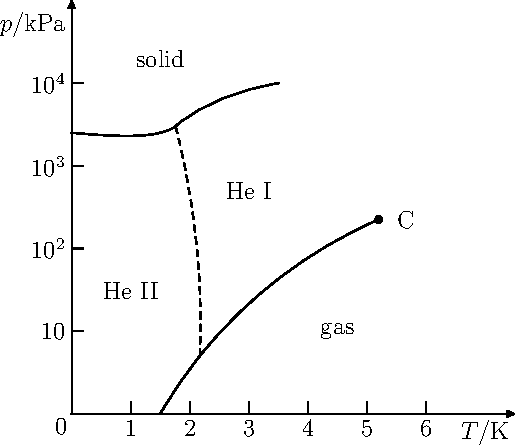
\includegraphics[width=0.45\textwidth]{graphics/phase_diag}
	\caption{The pressure-temperature phase diagram of $\He$. At atmospheric pressure and a temperature of $4.2\unit{K}$, $\He$ condenses into a liquid, known as He-I. As we cool further, helium becomes a superfluid, denoted as He-II on the phase diagram, below $T_{\lambda} \approx 2.17\unit{K}$. From the phase diagram, one will note that even at absolute zero, helium does not become solid. This is due to the weak van der Waals interaction between helium atoms and the fact that the zero-point oscillations of the helium atoms are so strong, that no solid is stable unless pressurized to above $2.5\unit{MPa}$.}
	\vspace{0.5cm}
	\label{phase}
\end{figure}

While the properties and behaviour of He-I are similar to classical viscous fluids, He-II exhibits significantly different properties. For example, the thermal conductivity is amongst the highest of any known material. Later, in 1937 Pyotr Kapitsa\cite{kapitsa} conducted a few experiments on superfluid flow through narrow capillaries. He observed that He-II was able to flow with negligible viscosity. This research was also recognized by a Nobel prize in 1978.

The phenomenological description of these effects, the \textit{two-fluid model}, was provided by Tisza and Landau. Together with the theory of Bose-Einstein condensation and quantum mechanics, these theories provide a basic understanding of superfluidity.

Moreover, superfluidity allows for the existence of vortices with discretely quantized circulation. These vortices are composed of circulating superfluid around a narrow core and can tangle to produce quantum turbulence (QT). QT is measurable using specific experimental methods, some of which will be described later in this work.




\newpage
\chapter{Theoretical Background}

The theoretical part of this Thesis is composed of three chapters:

\begin{itemize}
	\item[1.] The first serves as a brief introduction to the topic of superfluidity using  Bose-Einstein statistical physics and basic hydrodynamics.
	
	\item[2.] The second chapter focuses on macroscopic quantum effects of superfluids, and introduces the concept of quantized vortices using quantum mechanics.
	
	\item[3.] The last theoretical chapter deals with fluid dynamics; particularly the drag coefficients for various structures in fluid flows. We will also introduce the Reynolds number for oscillating objects immersed in both classical and quantum fluids.
\end{itemize}
All of the ideas discussed in this chapter can be found in standard textbooks \cite{skrbek}, \cite{landau} except for the derivation of the vortex line density at the end of second part, where the original papers of Feynman, Vinen and Hall are required \cite{feynman}, \cite{vinen1}, \cite{vinen2}.

\vspace{1cm}
{\Huge \bfseries Superfluidity}
\addcontentsline{toc}{chapter}{Superfluidity}
\vspace{0.3cm}


Among all chemical substances, helium is special and unique at low temperatures. Under normal conditions (room temperature and atmospheric pressure), helium gas behaves as an ideal gas and the most common isotope is $\He$, formed by 2 protons, 2 neutrons and 2 electrons.\footnote{There is another stable isotope of Helium, ${}^3\mathrm{He}$, which has one less neutron in the nucleus. In this Thesis, we will only focus on the isotope $\He$.} Due to the composition of the $\He$ atom, the resulting nuclear spin is equal to zero. Therefore, $\He$  is a boson and obeys Bose-Einstein quantum statistics. This will be discussed in more detail in {\sffamily\textbf{Section 1.1}}.

When cooled below $ T_{\lambda}=2.17\unit{K} $, $\He$ undergoes a second-order phase transition to the superfluid state and quantum effects become much more significant. Since the quantum mechanical wave function for bosons is symmetric, two arbitrary atoms can occupy the same quantum state. The Pauli exclusion principle does not apply to bosons, so the global state of He-II at low temperatures can be described as a considerable amount of particles sitting in the energy ground state.

We can therefore describe the whole He-II fluid as two inter-penetrating fluids, one composed of ground-state particles (and described by the macroscopic wave function) - the condensate or superfluid component, and a second classical-like fluid composed of thermally excited atoms - the normal fluid component. In the following sections, this \emph{two-fluid model} will be used to describe the rotational motion of the superfluid and consequently, the existence of quantum turbulence.

\newpage

\section{Helium-II as a Bose-Einstein Condensate}
The total spin of $\He$ is zero, so gaseous helium may be classified as a Bose gas. Additionally, if we assume no interactions between the particles, we may use the \textit{ideal Bose gas} model. This of course cannot provide a perfect description of helium's behaviour (due to its weak interactions), but it will suffice. The thermodynamic limit of the ideal Bose model provides an intuitive insight to helium's special properties, such as superfluidity.

\subsection*{Quantum Statistics}

We choose to work with a scaled inverted temperature $\beta\equiv 1/kT $ and chemical potential $\mu$, denoting the number of particles sitting in the state $\vert n\>$ as $N_n$ and corresponding energy as $\eps_n$.\footnote{The entire set of energies are positive $\{\eps_n\} > 0$ except for the ground state, for which we choose $\eps_0 = 0$.} 
A mathematical description of such a quantum system can be done through Bose-Einstein statistics. In this statistical model of a grand canonical ensemble, a given state can be independently occupied by an arbitrary number of particles. Hence, we write the grand canonical potential $ \Phi $ as:


\begin{equation}
\Phi (T, V, \mu) 
=-\beta^{-1} \ln \bigg[\displaystyle \prod_{n}
  \displaystyle \sum_{N_n=0}^{\infty}
  e^{-\beta N_n (\eps_n - \mu) } \bigg]
= \beta^{-1} \displaystyle \sum_{n} \ln (1 - e^{-\beta (\eps_n - \mu)})\,,
\label{partition}
\end{equation}

where we assumed $\mu<0$ for the purpose of convergence. If we think of each particle as a de Broglie wave with wavelength $\lambda \sim \hbar/p \sim \hbar/(\eps m)^{1/2}$, one can calculate the mean value of the total number of particles sitting in all thermal levels by replacing the sum with an integral over all possible wave numbers:

\begin{equation}
\<N\> = -\frac{\partial\Phi}{\partial\mu} 
= \sum_n \frac{1}{e^{\beta(\eps_n-\mu)}-1}
\approx
\frac{V}{(2\pi)^3}\int \text{d}^3k \frac{1}{e^{\beta(\eps_k-\mu)}-1} + N_0\,,
\label{integral}
\end{equation}

where the term $N_0$, representing the number of ground state particles, has been added as a correction. 
By integrating (\ref{integral}), this correction appears to be relevant only when the temperature of system reach the critical value (as shown in \cite{tong}):

\begin{equation}
T_c = \frac{2\pi \hbar^2}{mk} \bigg ( \frac{N}{V \zeta(3/2)}\bigg)^{2/3}\,,
\label{tc}
\end{equation}

where $\zeta(3/2)\approx 2.612$ is the value of Riemann zeta-function. If we substitute to (\ref{tc}) the values of $ N, V$ and $ m $, specific for $ \He $, we would predict that the critical temperature  should be $ T_c \approx 3.15\unit{K} $, which is not far from the observed superfluid transition at $ T_{\lambda} = 2.17 \unit{K} $. 

As temperature $T<T_c$ decreases, more and more particles, a macroscopic number $N_0$, will occupy a single quantum state and form the so-called \textit{Bose-Einstein condensate}.


\subsection*{Heat Capacity}
More evidence proving the close relation between superfluidity of $ \He $  and Bose-Einstein condensation is the behaviour of the heat capacity around the critical temperature.

\begin{wrapfigure}{r}{0.48\textwidth}
\vspace{-0.7cm}
\centering
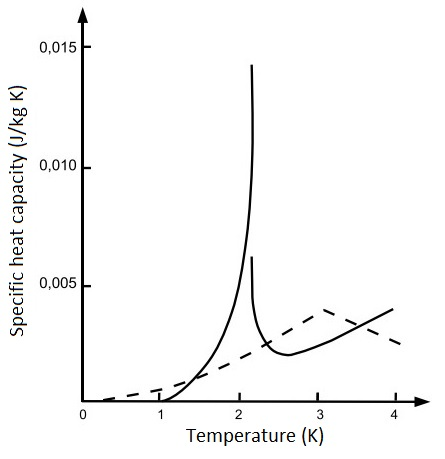
\includegraphics[width=0.48\textwidth]{graphics/capacity_bec}
\caption{Heat capacity of an ideal BEC (dashed line) and that measured for $\He$ (full line) as a function of temperature.}
\vspace{-0.5cm}
\end{wrapfigure}
From figure {\sffamily\textbf{Figure 1.1}} one can see that derivatives of both heat capacities (predicted by BEC and observed using $ \He $) are not continuous around critical temperatures $(T_c, T_{\lambda})$. Such discontinuities are often one of the characteristic properties of a phase transition in an infinite system. Since heat capacity is partial derivative of energy $ C_V = \partial E /\partial T \big\vert_V $, the second derivative would be discontinuous in this case, so therefore we classify the transition to the superfluid state as a $2^{\unit{nd}}$ order phase transition. Note that the shape of heat capacity plot as a function of temperature is reminiscent of the Greek letter $ \lambda $. This is the reason we call the superfluid transition   \textit{the $ \lambda$-transition} and denote the transition temperature as $ T_{\lambda}$. 

Transition to a superfluid phase can be also found in ${}^3\!\unit{He}$ (a fermion) at much lower temperatures $ \sim 1 \unit{mK} $. Although fermions cannot condense, they can form \textit{Cooper pairs}, in analogy with superconductors. These bound states are effectively bosons and therefore can undergo condensation.






\section{Two-Fluid Model}

Observations of superfluid helium led Tisza\cite{tisza} and Landau\cite{landau} to postulate their own theories describing the phenomena. Both assumed that macroscopically the whole fluid is composed of two inter-penetrating fluids. We recognize them as a \textit{normal} and pure \textit{superfluid} component with respective densities $ \rho_{\ind n} $, $\rho_{\ind s} $ and velocity fields  $\vec{v}_{\ind n} $, $ \vec{v}_{\ind s} $. At low relative velocities, the behaviour of both fluids can be considered as independent. However, the two components can interact through so-called \textit{mutual friction}, which will be discussed later in this work.

The total density $\rho$ can be written as the sum of the normal $\rho_{\ind n}$ and superfluid $\rho_{\ind s}$ components:

$$\rho = \rho_{\ind n} + \rho_{\ind s}\,.$$

The densities $ \rho_{\ind n} $, $\rho_{\ind s} $ vary with temperature due to decreasing mean value of statistical thermal excitations with reduced temperature. In 1947, L.D. Landau proposed\cite{landau_superfluid} the full microscopic theory of He-II from which the temperature dependence of the superfluid density was found to be given by $\rho_{\ind s}\!\propto\! -T^3$ below $0.6\unit{K}$ and $\rho_{\ind s}\!\propto\! -T^{1/2} e^{-\eps/T}$ at higher temperatures.

The first experiment proving Landau's theory was done by Andronikashvili\cite{andro}. He submerged a stack of tightly packed discs forming a torsional oscillator in He-II  to determine the fractional densities from the periods of oscillations. The corresponding fractional densities are plotted in {\sffamily\textbf{Figure 1.2}}.

\begin{figure}[h]
\centering

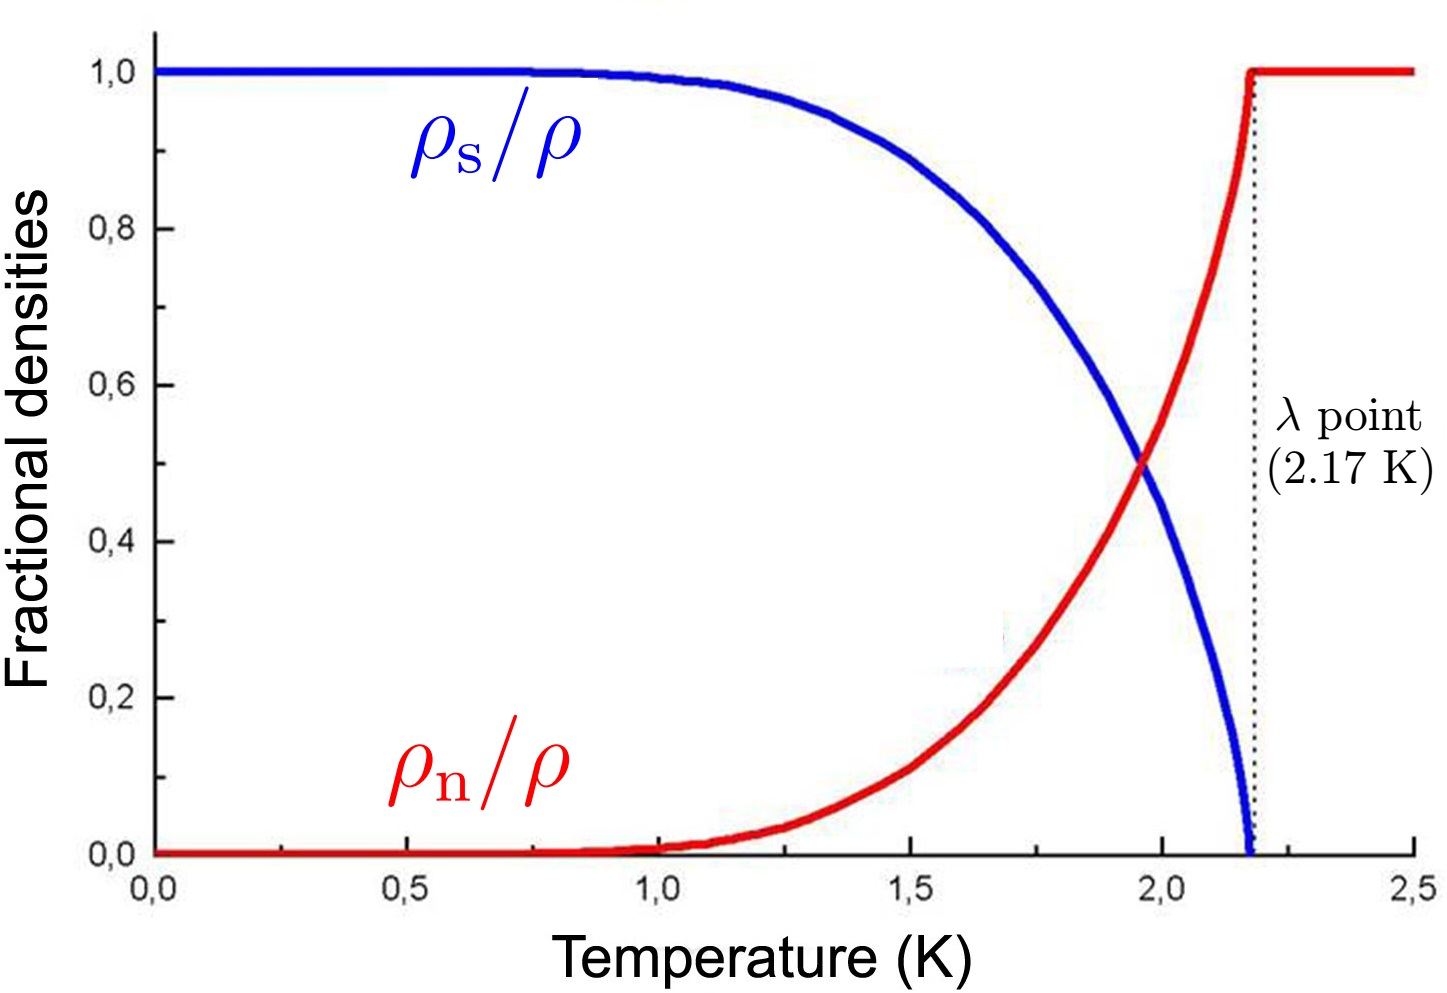
\includegraphics[scale=0.3]{graphics/densities}

\caption{Temperature dependence of fractional densities of the normal (red) and superfluid (blue) components. The total density $\rho$ varies only weakly with temperature.}
\end{figure}







\subsection*{Hydrodynamic Equations of the Two-Fluid Model}

Because we are working with more general forms of fluid motion, a generalised dynamic equation has to be derived, too. Due to incompressibility of the fluid and entropy conservation (assuming non-dissipative processes), the continuity equations must hold:

\begin{align}
\frac{\partial \rho}{\partial t}
=&
- \nabla \cdot (\rho_{\ind n} \vec{v_{\ind n}}
+ \rho_{\ind s} \vec{v_{\ind s}})
\label{cont_mass}\,,\\
\frac{\partial (\rho s)}{\partial t}=&
- \nabla \cdot (s\rho\vec{v_{\ind n}})\,.
\label{cont_entropy}
\end{align}

We are only missing the equations of motion for each of the two fluid components. They should have a form similar to the Navier-Stokes equation but with a few differences. We expect a mutual friction term, connecting both equations of motion, and a missing viscous term within the equation for the superfluid component.

The full derivation of the two-fluid equations of motion is fairly complicated and can be found in standard low temperature physics textbooks (such as \cite{skrbek}).

\newpage

The most general form of the motion equations for both, the normal and superfluid component, respectively are:

\begin{align}
\rho_{\ind n} \bigg [\frac{\partial\vec{v_{\ind n}}}{\partial t}
+ (\vec{v_{\ind n}}\cdot \nabla)\vec{v_{\ind n}} \bigg ]
=& -\frac{\rho_{\ind n}}{\rho} \nabla P
- \rho_s S \nabla T
- \frac{\rho_{\ind n}\rho_{\ind s}}{2\rho}
\nabla (\vec{v_{\ind n}}-\vec{v_{\ind s}})^2
+ \vec{F_{\ind {ns}}}
+ \eta_\ind{n} \nabla^2 \vec{v_\ind{n}}\,,
\label{motion_normal}\\
\rho_{\ind s} \bigg [\frac{\partial \vec{v_{\ind s}}}{\partial t}
+ (\vec{v_{\ind s}}\cdot \nabla)\vec{v_{\ind s}} \bigg ]
=& -\frac{\rho_{\ind s}}{\rho} \nabla P
+ \rho_s S \nabla T
+ \frac{\rho_{\ind n}\rho_{\ind s}}{2\rho}
\nabla (\vec{v_{\ind n}}-\vec{v_{\ind s}})^2
- \vec{F_{\ind {ns}}}\,,
\hspace{15mm}
\label{motion_super}
\end{align}

where $P$ is the applied pressure and $\eta_n$ denotes the viscosity of the normal component. The terms containing $\nabla T$ and $\nabla (\vec{v_{\ind n}} - \vec{v_{\ind s}})^2$ can be viewed as additional pressure effects.

Considering the simplest case, no thermal flow ($\nabla T = 0$), counterflow ($\vec{v_{\ind n}} - \vec{v_{\ind s}} = \vec{0}$) nor mutual friction ($\vec{F_{\ind{ns}}} = \vec{0}$) is present, we have a classical hydrodynamic system. In fact, (\ref{motion_normal}) would reduce to the Navier-Stokes equation for a classical fluid and (\ref{motion_super}) to the Euler equation for an ideal fluid without viscosity. Consequently, the two-fluid model seems to be applicable as a macroscopic approach to the overall behaviour of superfluid $\He$.  

\section{Second Sound}

The two-fluid model has an important consequence for wave behaviour of He-II. If we combine the continuity equations (\ref{cont_mass}), (\ref{cont_entropy}) and the equations of motion (\ref{motion_normal}), (\ref{motion_super}), we obtain (the particular method can be found in \cite{varga}) two wave equations. The first one describes a classical pressure-density wave with a corresponding velocity $ u_1 $:

\begin{equation}
\frac{\partial^2 \rho}{\partial t^2} = u_1^2 \nabla^2 \rho
\hspace{2cm}
u_1 = \bigg( \frac{\partial P}{\partial \rho} \bigg)_S^{1/2}\,.
\label{1sound}
\end{equation}

The second wave equation describes \textit{second sound}, an entropy-temperature wave with a velocity $ u_2 $,  given by

\begin{equation}
\hspace{0.6cm}
\frac{\partial^2 s}{\partial t^2} = u_2^2 \nabla^2 s
\hspace{2cm}
u_2 = \bigg( \frac{\rho_{\ind s}}{\rho_{\ind n}} \frac{Ts^2}{C_p} \bigg )^{1/2}\,,
\label{2sound}
\end{equation}

where $C_p$ is the specific heat. The first equation (\ref{1sound}) represents an ordinary sound, when both fluids oscillate identically ($\vec{v_{\ind n}} = \vec{v_{\ind s}}$). On the contrary, the second wave equation (\ref{2sound}) describes a new wave process, specific to $ \He $, when the components oscillate in anti-phase ($\rho_{\ind s}\vec{v_{\ind n}} = -\rho_{\ind n}\vec{v_{\ind s}}$). Consequently, the total density $ \rho $ is constant at every point, but the relative densities $ \rho_{\ind n} $, $ \rho_{\ind s} $ oscillate. This, consequently, can be viewed as the oscillation of temperature

In our work, the only significant changes in second sound velocity occur as we approach the lambda transition from below. At temperatures above $2.0 \unit{K}$, the second sound velocity starts to drop rapidly and tends towards zero at the lambda point.

\newpage














{\Huge \bfseries Quantum Effects}
\addcontentsline{toc}{chapter}{Quantum Effects}
\vspace{1cm}

As we may have seen in the previous chapter, the macroscopic behaviour of He-II is well determined by quantum statistical physics and Landau's two-fluid model. Since the superfluid component flows without dissipation (carrying no entropy), and is (indirectly) related to the atoms in the quantum mechanical ground state, an analogy with electrons orbiting the atomic nucleus can be constructed. This analogy led London to suggest a \textit{macroscopic wave function} $\Psi (\vec{r},t)$ to describe the superfluid component.

\subsection*{Properties of $\Psi (\vec{r},t)$}

The wave function $\Psi (\vec{r},t)$ is in general complex and its quadratic norm describes the average number of atoms in the condensate per unit volume:
$\vert \Psi \vert^2 =\Psi^* \Psi= \rho_{\ind s}/m_4\,$, where $m_4$ is the mass of one $\He$ atom. The simplest form of $\Psi (\vec{r},t)$ is given as:

\begin{equation}
\Psi(\vec{r},t) = \sqrt{\frac{\rho_{\ind s}}{m_4}}\,
e^{i \phi (\vec{r},t)}\,,
\label{psi}
\end{equation}

where the phase $\phi (\vec{r},t)$ is an unknown scalar function of spatial coordinates and time. If the whole system is described by a single wave function, the statistical properties are the same and the phases are correlated for all superfluid atoms. We can find out more about the velocity field $ \vec{v}_{\ind s} $ by applying the momentum operator $\hat{\vec{p}} = \frac{\hbar}{i} \nabla$ on the wave function $\Psi (\vec{r},t)$:

\begin{equation}
\vec{v_{\ind s}}
= \frac{\vec{\hat{p}} \vert\Psi\>}{m_4\vert\Psi\>}
= \frac{\hbar}{i} \frac{\nabla e^{i \phi(\vec{r},t)}}{m_4 e^{i \phi(\vec{r},t)}}
= \frac{\hbar}{m_4} \nabla \phi (\vec{r},t)\,.
\label{v_s}
\end{equation}

According to (\ref{v_s}), the velocity field $\vec{v_{\ind s}}$ is proportional to the gradient of the scalar field $\phi (\vec{r},t)$, which means the superfluid flow is \textit{potential}\footnote{One can find an equivalent situation in celestial mechanics or electrostatics, where the gravitational and electric potentials can be defined.}.  Moreover, due to the vector calculus identity
$\nabla \times (\nabla \phi(\vec{r}))=0\,,$
it turns out that the velocity field $\vec{v_{\ind s}}$ is rotationless. To be more precise, all vorticity vectors equal zero in a simply connected region: $\omega_{\vec{v_{\ind s}}} \equiv \nabla \times \vec{v_{\ind s}} = \vec{0}$. The obvious conclusion is that there are no superfluid vortices.

However, this is contrary to observation. One particular experiment, made by Osborne\cite{osborne}, proved the zero vorticity theorem wrong and will be discussed in more detail later in this chapter. The main consequence is that under some circumstances, the condition of space simplicity in He-II might be violated by "holes" in superfluid space. This hole effect directly leads to quantized properties such as \textit{quantized circulation}.


\section{Quantized Vortices}

Now we will look at the concept of circulation in more detail. Mathematically, the circulation is a path integral of velocity field along some contour, let call it $\mathcal{C}$. Generally, $\mathcal{C}$ is an arbitrary closed curve in 3D space with corresponding infinitesimal tangent vectors $\unit{d}\vec{\boldsymbol{\ell}}$. Denoting circulation as $\Gamma$, we can do the calculation using superfluid velocity field $\vec{v_{\ind s}}$ from (\ref{v_s}):

\begin{equation}
\Gamma = \oint_{\mathcal{C}} \vec{v_{\ind s}} \cdot \unit{d}\vec{\boldsymbol{\ell}}
= \frac{\hbar}{m_4} \oint_{\mathcal{C}} \nabla \phi \cdot \unit{d} \vec{\boldsymbol{\ell}}\,.
\label{gamma}
\end{equation}

From this integral one can get many results, depending on the space connectivity enclosed by loop $ \mathcal{C} $. In the case of no singularities (singly connected region, $ \Psi(\vec{r},t)\neq 0 $), the calculation is trivial and yields zero\footnote{No singularities mean a simple-connectivity of space, so every contour $ \mathcal{C} $ may be tightened in a limit to single point. Using Stokes' theorem
$$\Gamma_0
= \oint_{\mathcal{C}_0} \vec{v_{\ind s}} \cdot \unit{d}\vec{\boldsymbol{\ell}}
= \iint_{\mathcal{S_{\mathcal{C}_0}}} (\nabla \times \vec{v_{\ind s}})\cdot\unit{d}\vec{S} = 0\,, $$
where we used the fact that $ \nabla \times \vec{v}_{\ind s} = \vec{0} $.
}. If singularities are present (multiply connected region), there have to be certain places, where $ \Psi = 0 $. However, the wave function $\Psi\!\propto\!\unit{exp}\{i\phi(\vec{r},t)\} $ must be defined uniquely everywhere in space. Hence the phase $\phi$ can change along the loop either by zero or any multiple of $2\pi$. Using the residue theorem from complex calculus we can immediately show that the circulation is quantized:

\begin{equation}
\Gamma
= \frac{\hbar}{m_4} \oint_{\mathcal{C}} \nabla \phi \cdot \unit{d} \vec{\boldsymbol{\ell}}
= \frac{\hbar}{m_4} (\phi_{2\pi} -\phi_0)
= \frac{\hbar}{m_4} 2\pi n
\equiv n \kappa\,,
\label{nkappa}
\end{equation}

where $\kappa$ is called the \textit{circulation quantum}: $\kappa \approx 10^{-7}\unit{m^2 \dot s^{-1}}$.

\begin{figure}[h]
\centering
\vspace{0.5cm}
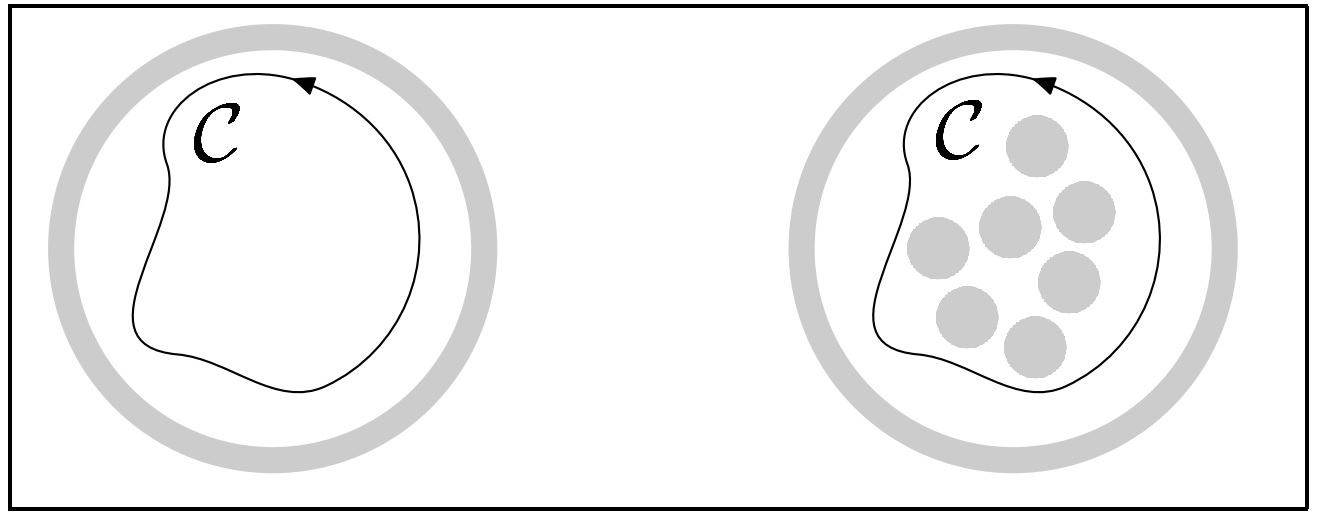
\includegraphics[width=0.8\textwidth]{graphics/singularity}
\caption{Sketch of singly connected region on the left and region containing singularities on the right, enclosed by loop $ \mathcal{C} $. We refer such singularities to the places, where identically $ \Psi = 0 $. In superfluid He-II, the multiple connected region correspond to the \textit{holes} in superfluid space - the places, where only the normal component is present.
}
\end{figure}


\newpage




\subsection*{Experiment Proving the Existence of Quantized Vortices in He-II}

In 1950, D.V. Osborne prepared an experiment \cite{osborne}, where a cylindrical container filled with He-II rotates around its principal axis. Since the superfluid component cannot rotate in the classical way, only the normal fluid should take the shape of a parabola. Classical mechanics predicts that the meniscus depth should be flatter as the density of liquid decreases. Surprisingly, Osborne did not observe any depth drop, even when the relative density of normal component was relatively small. 

\begin{wrapfigure}{l}{0.35\textwidth}
\vspace{-0.7cm}
\centering
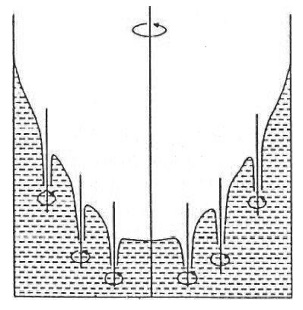
\includegraphics[width=0.35\textwidth]{graphics/rot_cont}
\vspace{-0.5cm}
\caption{A sketch of rotating container filled with He-II.}
\vspace{-0.5cm}
\end{wrapfigure}

A convincing explanation of this phenomenon was proposed by Richard Feynman\cite{feynman} predicting the existence of tiny superfluid vortices of discretely quantized circulation.
Such vortices ordered in an array within the bulk fluid can mimic macroscopic rotation. Quantitatively, if the angular velocity of the rotating container is $\vec{\Omega}$, then the classical vorticity is $ \omega = \nabla \times \vec{v} = 2\vec{\Omega} $ and the total circulation is - in the case of He-II - composed of circulation quanta $ \kappa $. From this we can define the \textit{vortex line density $ L $} as the number of quantized vortices intersecting a unit area, or in other words, the total length of all vortices per unit volume:

\vspace{-0.5cm}
\begin{equation}
\hspace{6cm}
L = \frac{2\Omega}{\kappa}\,.
\label{L}
\end{equation}



\subsection*{Basic Properties of a Single Quantized Vortex}

From the cylindrical symmetry we can find the velocity field near the vortex core:

\begin{equation}
\oint_{\mathcal{C}} \vec{v_{\ind s}} \cdot \unit{d}\vec{\boldsymbol{\ell}}
\stackrel{!}{=} n \kappa
\hspace{5mm}
\longrightarrow
\hspace{5mm}
\vec{v_{\ind s}} = \frac{\hbar}{m_4 r}n\, \vec{e_{\theta}}\,,
\label{v_r}
\end{equation}

where $\vec{e_{\theta}}$ is an unit vector perpendicular to the position vector $\vec{r}$. Near the vortex center, the velocity cannot be arbitrarily big. The highest value is given by the \textit{Landau critical velocity}\footnote{It is known\cite{tony} that exceeding the Landau critical velocity produces thermal excitations.} which is about $v_{\ind L} \approx 58 \unit{ms}^{-1}$ at zero pressure.
Thus, using (\ref{v_r})  we can estimate the radius of the core $a_0 = \hbar / m_4 v_L = 0.27 \unit{nm} \approx 3 \unit{\AA}$. A better estimate of $a_0$ by experiments shows that it is actually about $1 \unit{\AA}$.

We can also calculate the total energy per unit length of a single quantized vortex. This is obtainable by summing up the kinetic energy of the whole circulating superfluid component:

\begin{equation}
\eps_n
= \int_a^b \frac{1}{2} \rho_{\ind s} v_{\ind s}^2 2\pi r\unit{d}r
= \frac{\pi \hbar^2 \rho_{\ind s}}{m_4^2} n^2 \int_a^b \frac{\unit{d}r}{r}
= \frac{\pi \hbar^2 \rho_{\ind s} \ln(b/a)}{m_4^2}\, n^2
\equiv \eps_0 n^2\,,
\label{eps_n}
\end{equation}

where $\eps_0$ is the energy per unit length of a singly quantized vortex and $b$ is some characteristic length such as container length or the distance between two vortices. Here we can see that due to $E_{\ind{vortex}} \sim n^2$, it is energetically favourable to have singly quantized vortices.

\section{Quantum Turbulence}

Generally, quantized vortex lines do not need to be homogeneously distributed and fully polarized. In situations when these properties are considerably complex, the flow of the superfluid component is strongly chaotic. This randomisation of quantized vortices is known as  \textit{quantum turbulence}.

The two-fluid nature of superfluid $ \He $ definitely provides a more general form of motion of quantum fluids. Consequently, the understanding of such a remarkable physical system as quantum turbulence (QT), may turn to a deeper understanding of turbulence in classical fluids, which is, to this day, far from complete.


\subsection*{Mutual Friction}

Each vortex line is composed of the superfluid component rotating around a core of normal fluid. Hence, quantized vortices can interact with both components. In 1957, Vinen and Hall conducted several remarkable experiments\cite{vinen1} to observe this interaction. They measured how the presence of vortices affects the propagation of second sound waves and found out that vortex lines attenuate the second sound signal the same way friction does in the case of a linear mechanical oscillator. By this we mean that the damping is of the form $\sim\!\unit{exp}(-\alpha z)$, where $\alpha$ is the attenuation coefficient and $z$ is the chosen direction of the propagating wave. The attenuation effect was actually expected as the vortices and second sound both represent the relative motion of the two fluid components. Furthermore, the attenuation was found to be stronger when the rotational frequency $\Omega$ was increased or when the orientation of the propagating second sound wave was set to be more perpendicular to the vortices.

Combining all the observed properties together, Vinen and Hall laid the foundations\cite{vinen2} for the derivation of the following formula for the mutual friction force:

\begin{equation}
\vec{F}_{\ind{sn}}
= B \frac{\rho_{\ind n} \rho_{\ind s}}{\rho}
\hat{\vec{\Omega}}
\times [\vec{\Omega}\times(\vec{v}_{\ind n}
- \vec{v}_{\ind s})]
+ B^{\prime} \frac{\rho_{\ind n} \rho_{\ind s}}{\rho}
[\vec{\Omega}\times(\vec{v}_{\ind n} - \vec{v}_{\ind s})]\,.
\label{mutual}
\end{equation}

In (\ref{mutual}), the $\vec{\Omega}$ stands for the angular velocity of the rotating cryostat, $\hat{\vec{\Omega}}$ for its normalised vector, $(\vec{v}_{\ind n} - \vec{v}_{\ind s})$ for the velocity vector of second sound, $B$ and $B^{\prime}$ are (temperature-dependent) constants. The indices \text{\tt s,n} in $\vec{F}_{\ind{sn}}$ represent the case where the superfluid component acts on the normal component. As we might expect, mutual friction is antisymmetric with respect to the indices ($\vec{F}_{\ind{ns}} = - \vec{F}_{\ind{sn}}$).

\newpage

Now, let us replace the $\vec{\Omega}$ vector with $\vec{L}$ from (\ref{L}). Denoting $\theta$ as the angle between the vortex line density vector $\vec{L}$ and second sound velocity vector $\vec{v}_{\ind{ns}} = \vec{v}_{\ind n} - \vec{v}_{\ind s}$, and taking only the dissipative term of (\ref{mutual}) we obtain:

$$
\vec{F}_{\ind{sn}}
= -B \frac{\rho_{\ind n} \rho_{\ind s}}{2\rho} \kappa L
\vec{v}_{\ind{ns}} \sin^2\theta\,.
\label{mutual*}
$$

This simplification allows us to calculate an exact expression for the damping factor $\alpha$ of second sound. This formula contains the vortex line density $L$. Therefore, by measuring the damping factor $\alpha$ in an experiment, we can calculate $L$. This well-established technique is called the second sound attenuation.

\section{Second Sound Attenuation}

Now we have enough information to derive the attenuation factor of the second sound wave. Let us choose the \text{\tt z}-axis as the second sound wave's direction of propagation. Using (\ref{mutual*}) and equations of motion (\ref{motion_normal}), (\ref{motion_super}), the corresponding wave equation takes the form \cite{varga}:

\begin{equation}
\frac{\partial^2 \vec{v}_{\ind{ns}}}{\partial^2 z}
-
\frac{B\kappa L}{2 u_2^2}\sin^2\theta
\frac{\partial \vec{v}_{\ind{ns}}}{\partial t}
-
\frac{1}{u_2^2}
\frac{\partial^2 \vec{v}_{\ind{ns}}}{\partial^2 t}
=
0\,.
\label{ss_wave}
\end{equation}

Similar wave equations can be derived by considering for example a damped oscillator or electromagnetic waves in conducting medium. Inspired by Vinen and Hall observations, we seek the solution in the form of an exponentially damped wave:

\begin{equation}
\vec{v}_{\ind{ns}}
= v_0 e^{i(\omega t - kz)} e^{-\alpha z} \vec{e}_{\ind z}\,,
\end{equation}

where $e^{-\alpha z}$ is the damping factor and $v_0 e^{i(\omega t - kz)}\vec{e}_{\ind z}$ is a counterflow velocity wave propagating in the \text{\tt z}-direction with amplitude $v_0$, angular velocity $\omega$ and wave vector $k$. Substituting this result back into (\ref{ss_wave}) we obtain the following for the attenuation coefficient:

\begin{equation}
\alpha
= \frac{B\kappa L}{4 u_2} \sin^2 \theta\,.
\label{alpha}
\end{equation}

Of course, the distribution of vortex lines could be generally chaotic and unpredictable, and not only oriented at an angle $ \theta $. In a homogeneous and isotropic distribution, we choose rather to work with the mean value of $\sin^2{\theta}$ for all directions in 3D space, so the new attenuation constant $\alpha^*$ takes the form:

\begin{equation}
\alpha^*
= \frac{B\kappa L}{4 c_2} \< \sin^2 \theta \>
= \frac{B\kappa L}{6 c_2}
\label{alpha_mean}\,.
\end{equation}

As we can see, randomly distributed vortex lines attenuates 2/3-times less when compared with the perpendicular interaction with polarized vortices. 


\subsection*{Viscous Damping and Resonance Curve}

Mutual friction is not the only dissipative effect. While any amount of normal component is still present, classical viscous damping acts
even if no quantum turbulence is created. To account for this, the full attenuation should be composed of two constants:

\begin{equation}
\alpha = \alpha_0 + \alpha^*\,,
\label{attenuation}
\end{equation}

where $\alpha_0$ is the aforementioned viscous attenuation. Thus when the second sound signal is generated in a finite system, we measure the signal's characteristic resonance curve by changing the frequency. the resonance width $\Delta f$ of this resonator is related with $ \alpha $, $ \alpha_0 $ via:

\begin{equation}
\alpha_0 = \frac{\pi \Delta f_0}{u_2}
\hspace{2cm}
\alpha = \frac{\pi \Delta f}{u_2}\,,
\label{widths}
\end{equation}

where $\Delta f_0$ is the resonance width when no vortex lines are present. Taking out $L$ from (\ref{alpha_mean}) and using (\ref{attenuation}), (\ref{widths}) we get:

\begin{equation}
L
= \frac{6 c_2}{B \kappa} \alpha^*
= \frac{6\pi}{B\kappa} (\Delta f - \Delta f_0)\,.
\label{L_deltaf}
\end{equation}

The parameters $B$, $\Delta f_0$ and $\Delta f$ are measurable variables. However, there is a more practical way to measure certain quantities and then calculate $L$.

Second sound devices usually work on the basis of measuring a voltage across a biased resistive thermometer or across a capacitor made from a semi-permeable membrane placed in a second sound resonator. When on resonance, emitted second sound waves are reflecting back and forth, resulting in a standing wave formed in the resonator. The receiver observes a wave with an amplitude $A_0$ (when there are no vortices) and a decreased amplitude $A$, when a number of vortex lines are present.  The ratio of these amplitudes can be derived by summing up all the reflected waves and takes the form\cite{physrevB}:

\begin{equation}
\frac{A_0}{A}
= \frac{\Delta f}{\Delta f_0}\,.
\label{sums}
\end{equation}

Finally, connecting the results of (\ref{L_deltaf}) and (\ref{sums}) we obtain

\begin{equation}
L = \frac{6\pi \Delta f_0}{B\kappa}\bigg( \frac{A_0}{A} - 1 \bigg)\,,
\label{L}
\end{equation}

which allows us to determine the vortex line density by directly measurable parameters.


















\newpage

{\Huge \bfseries Fluid Dynamics}
\addcontentsline{toc}{chapter}{Fluid Dynamics}
\vspace{1cm}

Continuum equations cover processes occurring over a wide range of length scales, starting from quantized vortices ($10^{-10}\unit{m}$) to galactic motion ($10^{20}\unit{m}$). Under certain circumstances, the continuum flow may exhibit irregular, turbulent behaviour ({\sffamily\textbf{Figure 1.5}}, {\sffamily\textbf{Figure 1.6}} \cite{turbulence}).

Vortices were observed and painted by Leonardo da Vinci and since then, many theories have been developed but a general theory of turbulence remains elusive. In previous chapters, we introduced the basic properties of superfluid helium, which are governed by quantum mechanical effects. Since all quantized vortices are essentially identical, a description of quantum turbulence \textit{should be} relatively simpler and could lead to the development of a mathematical prototype of turbulence in general.

\begin{figure}[h]
\centering
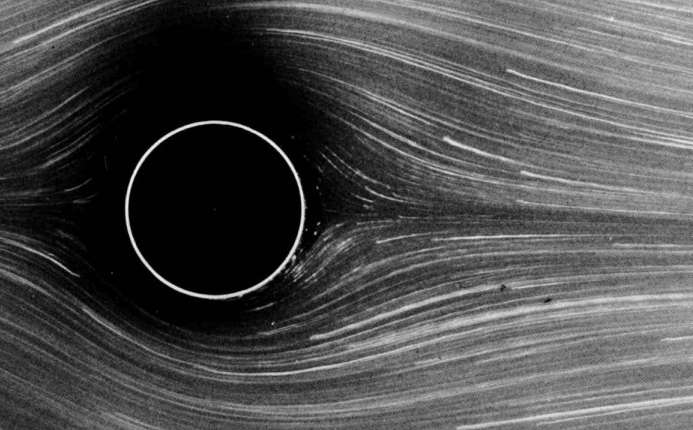
\includegraphics[width=0.6\textwidth]{graphics/laminar}
\caption{Photograph of laminar flow past a cylinder.}
\end{figure}

\begin{figure}[h]
\centering
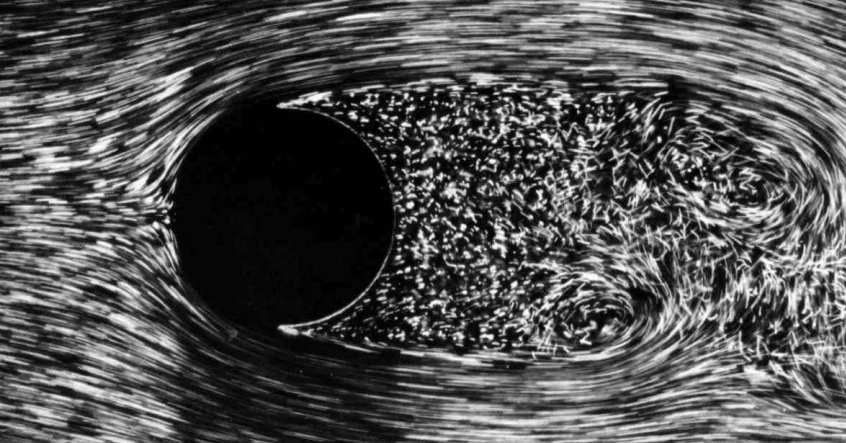
\includegraphics[width=0.6\textwidth]{graphics/turbulent}
\caption{Photograph of turbulent flow past a cylinder.}
\end{figure}

In the following sections, we will present a mathematical description of viscous fluids and their dynamics, focusing on the transition from laminar to turbulent flow and defining the dimensionless \textit{Reynolds number} (Re) and the drag coefficient $ C_D $. Finally, analogical hydrodynamic equations and properties will be defined for He-II as well. 

\newpage

\section{From Laminar to Turbulent Flow}

We define a flow as \textit{laminar} when the velocity field is steady in time and can be characterized by a set of non-intersecting streamlines. Turbulent flow displays chaotic dynamics, it contains vortices of various sizes and circulations and is therefore much harder to characterise than laminar flows. In fact, no exact definition exists.

Let us consider a classical Newtonian viscous fluid. Using the model of continuum physics one arrives\cite{landau} at the conservation of the mass, entropy and momentum (Navier-Stokes) equation, which completely determine the density, entropy and velocity fields $\vec{v}(\vec{r},t)$ of the fluid at any point in time or space:

\begin{align}
\frac{\partial \rho}{\partial t}
=& - \nabla \cdot (\rho\vec{v})\,,
\label{FD_mass}\\
\frac{\partial (\rho s)}{\partial t}
=& - \nabla \cdot (\rho s \vec{v})\,,
\label{FD_entropy}\\
\rho \bigg[ \frac{\partial\vec{v}}{\partial t}
+ (\vec{v}\cdot \nabla)\vec{v} \bigg ]
=& -\nabla P
+ \eta \nabla^2 \vec{v}
+ \rho\vec{f}\,,
\label{FD_NS}
\end{align}

where the last equation is valid only for incompressible fluids. In this case, the continuity equation can be reduced to $ \nabla \cdot \vec{v} = 0 $. Here $\rho$ denotes the fluid density, $\eta$ the dynamic viscosity and $\vec{f}$ sums up all external forces per unit mass. In addition, if we consider the flow as isotropic ($s = \unit{const}$), the entire fluid's motion is given by the reduced continuity equation and the Navier-Stokes equation (\ref{FD_NS}).

\subsection*{Principle of Dynamical Similarity and Reynolds Number}

In many cases, it is useful to transform the stationary $ (\partial \vec{v}/\partial t = \vec{0}) $ Navier-Stokes equation (\ref{FD_NS}) into a form containing dimensionless parameters. This can be done with the typical (mean) value of the flow velocity $\vec{v}_0$ and with the length scale $L$ at which the velocity changes most significantly. All magnitudes appearing in (\ref{FD_NS}) are scaled as:

$$
\vec{v^{\prime}} \equiv \frac{\vec{v}}{v_0} 
\hspace{5mm} \bigg\vert \hspace{5mm}
\vec{r}^{\prime} \equiv \frac{\vec{r}}{L}
\hspace{5mm} \bigg\vert \hspace{5mm}
\nabla^{\prime}  \equiv L\nabla
\hspace{5mm} \bigg\vert \hspace{5mm}
P^{\prime}       \equiv \frac{P}{P_0} = \frac{P}{\rho v_0^2}\,.
$$

After the substitution, we obtain the dimensionless Navier-Stokes equation. Assuming no external forces, after some algebraic manipulations we get:

\begin{equation}
(\vec{v}^{\prime}\cdot \nabla^{\prime})\vec{v}^{\prime}
= -\nabla^{\prime} P^{\prime}
+ \frac{\eta}{\rho v_0 L} {\nabla^{\prime}}^2 \vec{v}^{\prime}
\equiv -\nabla^{\prime} P^{\prime}
+ \frac{1}{\text{Re}} {\nabla^{\prime}}^2 \vec{v}^{\prime}\,.
\label{reynolds}
\end{equation}

Here, the Reynolds number is defined as the ratio of inertial and viscous dissipative forces  $\Re \sim (\vec{v}^{\prime}\cdot \nabla^{\prime})\vec{v}^{\prime} / {\nabla^{\prime}}^2 \vec{v}^{\prime}$ and can be expressed as $\Re = \rho v_0 L / \eta$. From this definition, we can conclude that all flows with the same $\unit{Re}$ and the same boundary conditions (similar, appropriately scaled geometries) have also the same dynamics, because they are represented by the same dynamical equation.

According to our definition, we can use the Reynolds number as an indicator as to whether or not a given steady flow of classical fluid is laminar or turbulent. In flow past a cylinder, the laminar character is observed when $\Re\sim 1$, and the very first laminar vortices appear in the wake when $\Re\sim 10$. Above this value, the viscous term starts to be much smaller compared to the inertial one and more and more kinetic energy is carried by the vortices.

When $\Re \sim 100$, the so-called \textit{K\'arm\'an vortex street} is observed before fully developed turbulence emerges at $\Re > 10^5$ (see in \cite{turbulence}). Here, the viscosity no longer plays any role at large length scales and most of the injected energy is transferred to very small vortices without much dissipation along the way. The kinetic energy is, of course, eventually dissipated by viscous forces acting at the smallest length scales (suppressing the motion of the smallest vortices).


\section{Drag Forces Acting on Submerged Objects}

Let us consider a fluid flowing past a solid object of some arbitrary shape. In the case of a viscous fluid, the \textit{drag force} acting on the bluff body depends on the flow velocity, viscosity and geometry of the object. For example, if we choose laminar flow past a sphere, then the relation for the viscous drag force\footnote{This type of drag force is sometimes called \textit{skin friction}.} is the famous Stokes' law:

\begin{equation}
\vec{F}_{\ind{lam}} = 6\pi \eta r \vec{v}\,,
\label{laminar}
\end{equation}

where $r$ is the radius of the sphere and $ \vec{v} $ is the velocity of the stream at infinity. Relation (\ref{laminar}) is specific for a sphere, but the proportionality $\vec{F}_{\ind{lam}}\!\propto\!\vec{v}$ holds for any arbitrary body.
When the Reynolds number is high enough, the drag force (or pressure drag) for a turbulent flow is expressed as:

\begin{equation}
\vec{F}_{\ind{turb}} = \frac{1}{2} C_D S \rho v^2 \vec{\hat{e}}_{\vec{v}}\,,
\label{turbulent}
\end{equation}

where $S$ is the cross-sectional area of the object perpendicular to the flow, $\vec{\hat{e}}_{\vec{v}}$ is a unit vector pointing in the same direction as $\vec{v}$ and $C_D$ is the \textit{drag coefficient}, which is a specific dimensionless number related with the body's geometry.
Henceforth, we will describe the fluid motion in terms of the drag coefficient dependence $C_D(v)$ on velocity instead of the force dependence $F(v)$.

In summary, the relation for laminar and turbulent (Newton) cases takes the form:
$$
C_D \!\propto\! v^\alpha, \hspace{1cm}
\text{where}
\left\{ 
  \begin{array}{l l}
    \alpha=-1 & \quad \text{for $\Re \in (0-10)$}\\
    \alpha=0 & \quad \text{for $\Re \in (10^3-10^5)$}
  \end{array}
\right.\,. 
$$

The full dependence of experimentally measured $C_D(\Re)$ (for constant density, viscosity and similar sizes of objects) is sketched on the graph below for various geometries.

\begin{figure}[h]
\centering
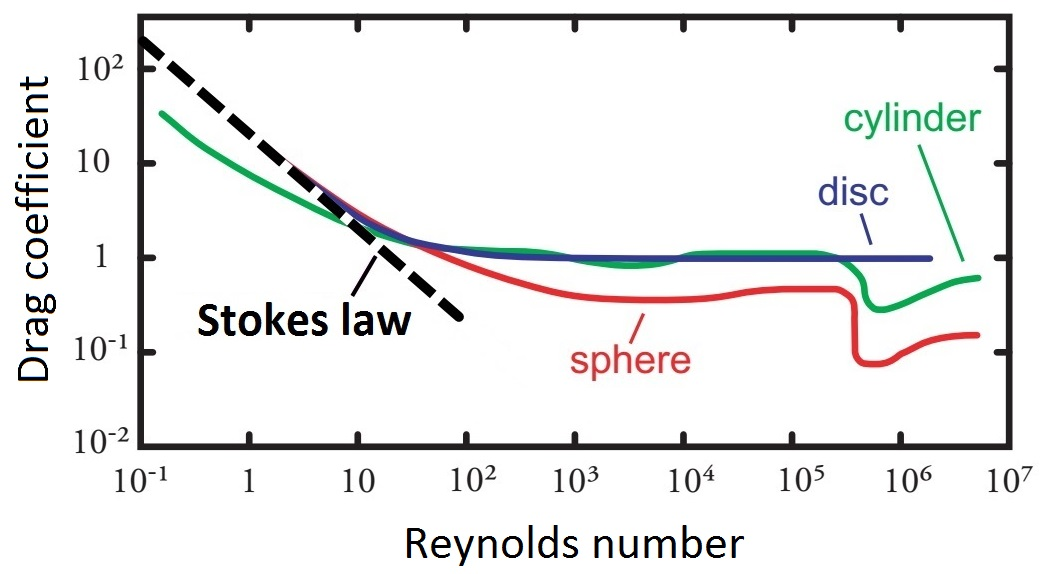
\includegraphics[scale=0.4]{graphics/dragcoeff}
\caption{Drag coefficient dependence for a thin disc (blue line), cylinder (green line) and a sphere (red line) versus the Reynolds number. In this log-log plot, the laminar drag (black line) is undoubtedly localised within low values of $\Re$ with known relation $C_D \!\propto\! \Re^{-1}$. Then, at $\Re \in (10^2-10^3)$, the pressure drag dominates and $C_D=\text{const.}$ until it suddenly falls down at $\Re \approx 500,000$. This phenomenon is called the \textit{drag crisis}, which states that above the critical value of $\Re$, the boundary layer around the object turns turbulent and therefore, the separation region (the region where the boundary layer detaches from the surface of the bluff body) shifts, reducing the cross-section of the turbulent wake. Note that this does not occur for the thin disc (placed perpendicularly to the flow).}
\end{figure}



\section{Oscillatory Motion in a Viscous Fluid}

Since this work concerns vibrating objects (tuning forks) in superfluid He-II, we will briefly discuss the theory of oscillatory fluid behaviour.

\subsection*{Penetration Depth} 

If an infinite \text{\tt xy}-plane is submerged in a viscous fluid and harmonically oscillating in \text{\tt x}-direction with angular frequency $\omega$, the fluid will also oscillate in the \text{\tt x}-direction with the same frequency as the plane does due to viscous forces. However, the dissipative processes will damp the oscillation as we go further from the plane in the \text{\tt z}-direction (plane is put at $z=0$). Hence we are expecting the solution of Navier-Stokes equation (\ref{FD_NS}) in the
form of $ \vec{v} = \big[ v_x(z,t), 0, 0 \big] $. The motion equation is in this case much simpler, because the term $ (\vec{v}\cdot \nabla)\vec{v} = 0 $, the pressure is constant everywhere $ P=\text{const.} $ and gravitational force
can be neglected. 

\newpage

For this situation, the solution of Navier-Stokes equation (\ref{FD_NS}) is a well-known exponentially attenuated harmonic wave:

\begin{equation}
\vec{v} = v_0 e^{i(kz - \omega t)} e^{-z/\delta} \vec{\hat{e}}_{\ind z}\,,
\label{v_pen}
\end{equation}

where $k = 1/\delta$ is the wave number, and $\delta$ is the \textit{penetration depth}. Beyond this distance, the fluid oscillation is damped stronger than $e$-times, so $ \delta $ becomes the characteristic dimension of the damped wave. It is given as\cite{landau}:

\begin{equation}
\delta = \sqrt{\frac{2\eta}{\rho \omega}}\,.
\label{penetration}
\end{equation}

The penetration depth decreases with frequency, meaning that for high-frequency oscillations, the fluid oscillations are confined to the vicinity of the oscillating plane.

\subsection*{Oscillatory Reynolds Number}

Because of the extra degree of freedom in oscillatory flow (the period of oscillation), one dimensionless parameter such as Re, as defined for steady flow, cannot fully describe the flow. Hence, two dimensionless numbers are generally needed. 

However, in the special case of the \textit{high-frequency limit} ($ \omega > 2\eta / \rho L^2  $) the situation is simplified. If the penetration depth $ \delta $ becomes significantly smaller than all other relevant dimensions such as body size or surface roughness, then $ L $ should be replaced by $ \delta $ in the process of scaling the Navier-Stokes equation. This is because one of the points of the scaling is to estimate the magnitudes of velocity derivatives in the flow field and we have to take the largest values available. From this re-scaling of the NS equations it follows that in the high frequency limit, all relevant quantities can be again combined into a single dimensionless parameter -- the oscillatory Reynolds number $ \Re_{\delta} $. Using (\ref{penetration}) we obtain:

\begin{equation}
\Re_{\delta} = \frac{v_0 \delta\rho}{\eta}
= v_0 \sqrt{\frac{\rho}{\eta \pi f}} \,.
\label{Re*}
\end{equation}

\section{Oscillations in Superfluid He-II}

So far, have only considered oscillations in a classical fluid. To apply the theory to two-fluid model, we have to make adjustments so that it will work for both the normal and superfluid component. 

When a high-frequency oscillating body with low velocity amplitude is submerged in superfluid He-II, the drag force is expected to be caused only by the viscous forces of the normal component. However, the density $ \rho_{\ind n} $ of this component decreases with temperature (as introduced in {\sffamily\textbf{Section 1.2, Figure 1.2}}) and we are forced to work with the characteristic penetration depth $\delta_{\ind n}$ and oscillatory Reynolds number $\Re_{\ind n}$:

\begin{equation}
\delta_{\ind n} = \sqrt{\frac{2\eta}{\rho_{\ind n}\omega}}\,,
\hspace{1cm}
\Re_{\ind n} = \frac{v_0 \delta_{\ind n} \rho_{\ind n}}{\eta}
\label{twofluid}\,.
\end{equation}



\begin{figure}[h]
	\centering
	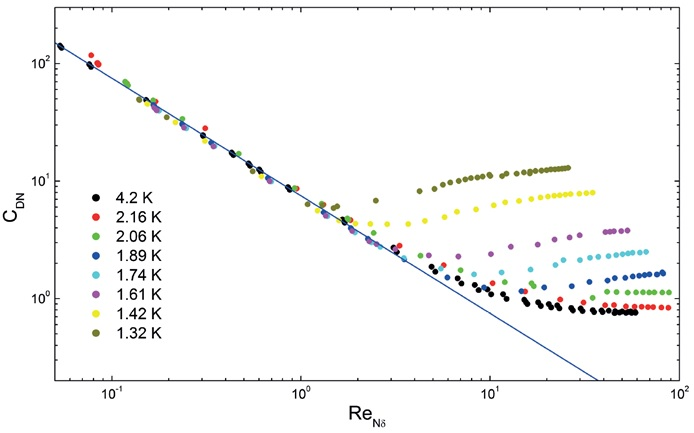
\includegraphics[width=0.75\textwidth]{graphics/C_Re}
	\caption{Number of experiments made a few years ago show that the definition of oscillatory Reynolds number in superfluid $ \He $ (\ref{twofluid}) is chosen correctly since all curves lies on the same place within the laminar range and in turbulent differs only by the presence of QT. }
\end{figure}



\subsection*{Motivation}

The drag coefficient for objects submerged in classical fluids have been explored already. The process and conditions for making the turbulence have been intensively studied for various-shaped objects and wide range of oscillation frequencies.
 
Because of two-fluid behaviour of He-II, two types of turbulence may occur when an immersed body oscillates - classical and quantum. The first one is an ordinary turbulence caused by the normal component and described by the oscillatory Reynolds number $ \Re_{\delta} $.
The second, quantum turbulence consists of quantized vortices, for which the complete theoretical description and sufficient number of experiments are still missing, but there are hints that the relevant physical quantity governing vortex nucleation is a critical velocity, which is expected to scale as $\sqrt{\omega \kappa}$ \cite{schoepe}, where $\omega$ is angular frequency and $\kappa$ the circulation quantum.
 
We already know that vortex nucleation can be launched if the normal component or a submerged body moves at a high enough velocity relative to the superfluid component, but to this day, experiments are missing that would clearly prove whether both turbulences form simultaneously or not. In this work we present measurements showing that classical and quantum turbulence can form independently. 